\paragraph{}
Le package RGtk2 s'ajoute en tant que librairie externe pour inclure dans R la possibilité de créer des interfaces graphiques. 

\paragraph{}
Comme dans Explorer3d, on a besoin de gérer les données grâce à l'interface graphique. Cette extension de R est essentielle dans le développement de l'application. 

 \begin{center}
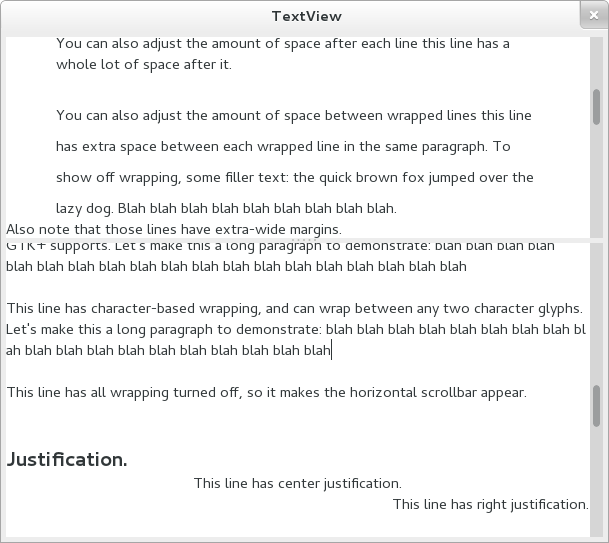
\includegraphics[scale=0.4]{multipleviews.png}\\
\textit{fenêtre divisée en plusieurs parties}
\end{center}

\paragraph{}
RGtk est un package dérivé de GTK2. Il est écrit en c++. GTK est un standard pour la création d'interface utilisateurs en c++ et bien d'autres langages. Grâce à RGtk2 nous pouvons résoudre le problème de création d'interface graphique. Comme dans la capture d’écran précédente nous pouvons créer une fenêtre avec plusieurs compartiments à l’intérieur de celle ci. Nous pouvons aussi avoir une fenêtre pour choisir la couleur d’un objet affiché dans une vue RG.

\begin{center}
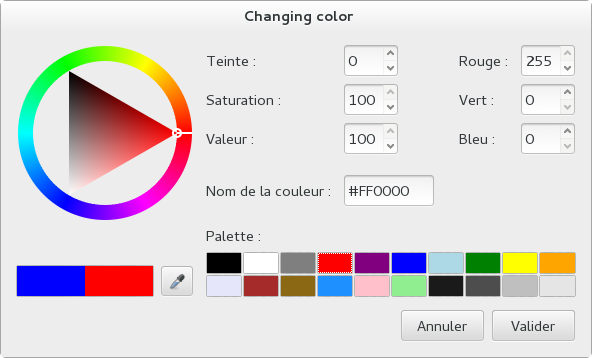
\includegraphics[scale=0.4]{colorselector2.png}\\
\textit{Sélectionneur de couleur RGtk}
\end{center}

\paragraph{}
Le but de RGtk2 est de surcoucher GTK. Avec ce package on pourra interagir avec le logiciel. \\\\\indent

Ce package nous offre la possibilité de créer
des interfaces graphiques pour l’utilisateur, ce qui lui permettra de faire les
demandes de calculs, sans passer par la console.\\

\begin{center}
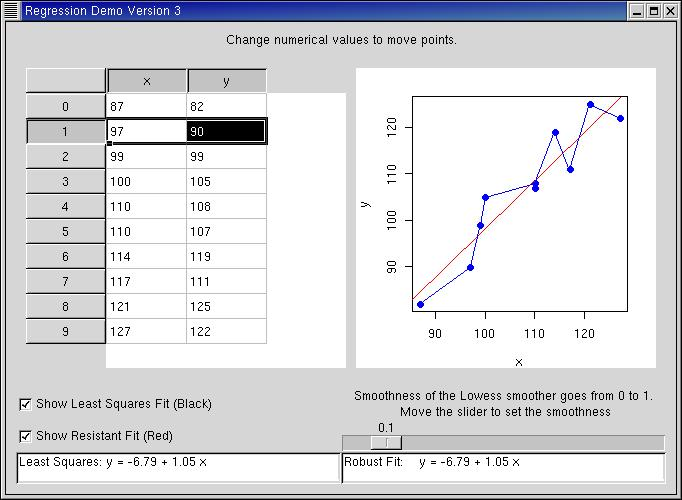
\includegraphics[scale=0.4]{regression.jpg}\\
\textit{Un autre exemple d'interface graphique avec RGtk}
\end{center}